%% For double-blind review submission, w/o CCS and ACM Reference (max submission space)
\documentclass[sigplan]{acmart}\settopmatter{printfolios=true,printccs=false,printacmref=false}
%\settopmatter{authorsperrow=2}
%% For double-blind review submission, w/ CCS and ACM Reference
%\documentclass[sigplan,review,anonymous]{acmart}\settopmatter{printfolios=true}
%% For single-blind review submission, w/o CCS and ACM Reference (max submission space)
%\documentclass[sigplan,review]{acmart}\settopmatter{printfolios=true,printccs=false,printacmref=false}
%% For single-blind review submission, w/ CCS and ACM Reference
%\documentclass[sigplan,review]{acmart}\settopmatter{printfolios=true}
%% For final camera-ready submission, w/ required CCS and ACM Reference
%\documentclass[sigplan]{acmart}\settopmatter{}


%% Conference information
%% Supplied to authors by publisher for camera-ready submission;
%% use defaults for review submission.
\acmConference[]{Project Report}{November 15, 2018}{Runtime Verification, Inc.}
\acmYear{2018}
\acmISBN{} % \acmISBN{978-x-xxxx-xxxx-x/YY/MM}
\acmDOI{} % \acmDOI{10.1145/nnnnnnn.nnnnnnn}
\startPage{1}

%% Copyright information
%% Supplied to authors (based on authors' rights management selection;
%% see authors.acm.org) by publisher for camera-ready submission;
%% use 'none' for review submission.
\setcopyright{none}
%\setcopyright{acmcopyright}
%\setcopyright{acmlicensed}
%\setcopyright{rightsretained}
%\copyrightyear{2018}           %% If different from \acmYear

%% Bibliography style
\bibliographystyle{ACM-Reference-Format}
%% Citation style
%\citestyle{acmauthoryear}  %% For author/year citations
%\citestyle{acmnumeric}     %% For numeric citations
%\setcitestyle{nosort}      %% With 'acmnumeric', to disable automatic
                            %% sorting of references within a single citation;
                            %% e.g., \cite{Smith99,Carpenter05,Baker12}
                            %% rendered as [14,5,2] rather than [2,5,14].
%\setcitesyle{nocompress}   %% With 'acmnumeric', to disable automatic
                            %% compression of sequential references within a
                            %% single citation;
                            %% e.g., \cite{Baker12,Baker14,Baker16}
                            %% rendered as [2,3,4] rather than [2-4].


%%%%%%%%%%%%%%%%%%%%%%%%%%%%%%%%%%%%%%%%%%%%%%%%%%%%%%%%%%%%%%%%%%%%%%
%% Note: Authors migrating a paper from traditional SIGPLAN
%% proceedings format to PACMPL format must update the
%% '\documentclass' and topmatter commands above; see
%% 'acmart-pacmpl-template.tex'.
%%%%%%%%%%%%%%%%%%%%%%%%%%%%%%%%%%%%%%%%%%%%%%%%%%%%%%%%%%%%%%%%%%%%%%


%% Some recommended packages.
\usepackage{booktabs}   %% For formal tables:
                        %% http://ctan.org/pkg/booktabs
\usepackage{subcaption} %% For complex figures with subfigures/subcaptions
                        %% http://ctan.org/pkg/subcaption

\usepackage{listings}
\usepackage{tikz}
\usetikzlibrary{positioning}
\usetikzlibrary{graphs}

% colors
\definecolor{shadecolor}{gray}{1.00}
\definecolor{darkgray}{gray}{0.30}
\definecolor{violet}{rgb}{0.56, 0.0, 1.0}
\definecolor{forestgreen}{rgb}{0.13, 0.55, 0.13}

% Col language definition
\lstdefinelanguage{Coq} {
mathescape=true,						
texcl=false,
morekeywords=[1]{
  Add,
  All,
  Arguments,
  Axiom,
  Bind,
  Canonical,
  Check,
  Close,
  CoFixpoint,
  CoInductive,
  Coercion,
  Contextual,
  Corollary,
  Defined,
  Definition,
  Delimit,
  End,
  Example,
  Export,
  Fact,
  Fixpoint,
  Goal,
  Graph,
  Hint,
  Hypotheses,
  Hypothesis,
  Implicit,
  Implicits,
  Import,
  Inductive,
  Lemma,
  Let,
  Local,
  Locate,
  Ltac,
  Maximal
  Module,
  Morphism,
  Next,
  Notation,
  Obligation,
  Open,
  Parameter,
  Parameters,
  Prenex,
  Print,
  Printing,
  Program,
  Projections,
  Proof,
  Proposition,
  Qed,
  Record,
  Relation,
  Remark,
  Require,
  Reserved,
  Resolve,
  Rewrite,
  Save,
  Scope,
  Search,
  Section,
  Show,
  Strict,
  Structure,
  Tactic,
  Theorem,
  Unset,
  Variable,
  Variables,
  View,
  inside,
  outside
},
morekeywords=[2]{
  as,
  cofix,
  else,
  end,
  exists,
  exists2,
  fix,
  for,
  forall,
  fun,
  if,
%  in,
  is,
  let,
  match,
  nosimpl,
  of,
  return,
  struct,
  then,
  vfun,
  with
},
morekeywords=[3]{Type, Prop, Set, True, False},
morekeywords=[4]{
  after,
  apply,
  assert,
  auto,
  bool_congr,
  case,
  change,
  clear,
  compute,
  congr,
  cut,
  cutrewrite,
  destruct,
  elim,
  field,
  fold,
  generalize,
  have,
  heval, 
  hnf,
  induction,
  injection,
  intro,
  intros,
  intuition,
  inversion,
  left,
  loss,
  move,
  nat_congr,
  nat_norm,
  pattern,
  pose,
  refine,
  rename,
  replace,
  revert,
  rewrite,
  right,
  ring,
%  set,
  simpl,
  split,
  suff,
  suffices,
  symmetry,
  transitivity,
  trivial,
  unfold,
  unlock,
  using,
  without,
  wlog,
  autorewrite
},        
morekeywords=[5]{
  assumption,
  by,
  contradiction,
  done,
  exact,
  lia,
  gappa,
  omega,
  reflexivity,
  romega,
  solve,
  tauto,
  discriminate,
  unsat
},
morecomment=[s]{(*}{*)},
morekeywords=[6]{do, first, try, idtac, repeat},
showstringspaces=false,
morestring=[b]",
% Size of tabulations
tabsize=3,							
% Enables ASCII chars 128 to 255
extendedchars=true,  		 		
% Case sensitivity
sensitive=true, 
% Automatic breaking of long lines
breaklines=false,
% Default style fors listings
%basicstyle=\scriptsize\ttfamily,
basicstyle=\footnotesize\ttfamily,
% Position of captions is bottom
captionpos=b,							
% Full flexible columns 
columns=[l]fullflexible,
% Style for (listings') identifiers
identifierstyle={\color{black}},
% Style for declaration keywords
keywordstyle=[1]{\color{violet}},
% Style for gallina keywords
keywordstyle=[2]{\color{forestgreen}},
% Style for sorts keywords
keywordstyle=[3]{\color{forestgreen}},
% Style for tactics keywords
keywordstyle=[4]{\color{blue}},
% Style for terminators keywords
keywordstyle=[5]{\color{red}},
%Style for iterators
keywordstyle=[6]{\color{violet}},
% Style for strings
stringstyle=,
% Style for comments
commentstyle=\it\ttfamily\color{brown},
% Style for lines numbering
numberstyle=\tiny,
literate={\\/}{{$\lor~$}}1
         {/\\}{{$\land~$}}1
         {<>}{{$\neq~$}}1
         {:->}{{$\mapsto~$\!}}1
         {\\->}{{$\mapsto~$\!}}1
         {<--}{{$\asgn~$}}1
         {\\in}{{$\in~$}}1
         {\\notin}{{$\notin~$}}1
         {++}{{$+\!+\!~$}}1
         {->}{{$\to~$}}1
         {forall}{{$\forall~$}}1
         {exists}{{$\exists~$}}1
         {=>}{{$\Rightarrow~$}}1
         {\\~}{{$\lnot\;$}}1
%         {\\+}{{$\!\join\!~$}}1
}

\lstdefinestyle{Coq}{language=Coq}
\lstset{language=Coq}


\begin{document}

%% Title information
\title{Verification of Casper in the Coq Proof Assistant}         %% [Short Title] is optional;
                                        %% when present, will be used in
                                        %% header instead of Full Title.
%\titlenote{with title note}             %% \titlenote is optional;
                                        %% can be repeated if necessary;
                                        %% contents suppressed with 'anonymous'
%\subtitle{Subtitle}                     %% \subtitle is optional
%\subtitlenote{with subtitle note}       %% \subtitlenote is optional;
                                        %% can be repeated if necessary;
                                        %% contents suppressed with 'anonymous'


%% Author information
%% Contents and number of authors suppressed with 'anonymous'.
%% Each author should be introduced by \author, followed by
%% \authornote (optional), \orcid (optional), \affiliation, and
%% \email.
%% An author may have multiple affiliations and/or emails; repeat the
%% appropriate command.
%% Many elements are not rendered, but should be provided for metadata
%% extraction tools.

%% Author with single affiliation.
\author{Karl Palmskog \quad Milos Gligoric}
%\authornote{with author1 note}          %% \authornote is optional;
%                                       %% can be repeated if necessary
%\orcid{nnnn-nnnn-nnnn-nnnn}             %% \orcid is optional
\affiliation{
  %\position{Position1}
  %\department{Department1}              %% \department is recommended
  \institution{The University of Texas at Austin}            %% \institution is required
  %\streetaddress{Street1 Address1}
  %\city{City1}
  %\state{State1}
  %\postcode{Post-Code1}
  %\country{USA}                    %% \country is recommended
}
\email{{palmskog,gligoric}@utexas.edu}          %% \email is recommended

\author{Brandon Moore}
\affiliation{
  %\position{Position1}
  %\department{Department1}              %% \department is recommended
  \institution{Runtime Verification, Inc.}            %% \institution is required
  %\streetaddress{Street1 Address1}
  %\city{City1}
  %\state{State1}
  %\postcode{Post-Code1}
  %\country{USA}                    %% \country is recommended
}
\email{brandon.moore@runtimeverification.com}          %% \email is recommended

%% Author with single affiliation.
\author{Lucas Pe{\~n}a}
%\authornote{with author1 note}          %% \authornote is optional;
                                        %% can be repeated if necessary
%\orcid{nnnn-nnnn-nnnn-nnnn}             %% \orcid is optional
\affiliation{
  %\position{Position1}
  %\department{Department1}              %% \department is recommended
  \institution{Runtime Verification, Inc.}            %% \institution is required
  %\streetaddress{Street1 Address1}
  %\city{City1}
  %\state{State1}
  %\postcode{Post-Code1}
  %\country{USA}                    %% \country is recommended
}
\email{lucas.pena@runtimeverification.com}          %% \email is recommended
\affiliation{
  %\position{Position1}
  %\department{Department1}              %% \department is recommended
  \institution{University of Illinois at Urbana-Champaign}            %% \institution is required
  %\streetaddress{Street1 Address1}
  %\city{City1}
  %\state{State1}
  %\postcode{Post-Code1}
  %\country{USA}                    %% \country is recommended
}
\email{lpena7@illinois.edu}          %% \email is recommended

\author{Grigore Ro{\c s}u}
\affiliation{
  %\position{Position1}
  %\department{Department1}              %% \department is recommended
  \institution{Runtime Verification, Inc.}            %% \institution is required
  %\streetaddress{Street1 Address1}
  %\city{City1}
  %\state{State1}
  %\postcode{Post-Code1}
  %\country{USA}                    %% \country is recommended
}
\email{grigore.rosu@runtimeverification.com}          %% \email is recommended
\affiliation{
  %\position{Position1}
  %\department{Department1}              %% \department is recommended
  \institution{University of Illinois at Urbana-Champaign}            %% \institution is required
  %\streetaddress{Street1 Address1}
  %\city{City1}
  %\state{State1}
  %\postcode{Post-Code1}
  %\country{USA}                    %% \country is recommended
}
\email{grosu@illinois.edu}          %% \email is recommended

%\shortauthors{Palmskog, Gligoric, Pe{\~n}a, and Ro{\c s}u}

%% Abstract
%% Note: \begin{abstract}...\end{abstract} environment must come
%% before \maketitle command
\begin{abstract}
This report describes our effort to model and verify the Casper blockchain
finality system in the Coq proof assistant.
We outline the salient details on blockchain systems using Casper, describe
previous verification efforts we used as a starting point, and give an overview
of the formal definitions and properties proved.
The Coq source files are available at:\\
\url{https://github.com/runtimeverification/casper-proofs}
\end{abstract}


%% 2012 ACM Computing Classification System (CSS) concepts
%% Generate at 'http://dl.acm.org/ccs/ccs.cfm'.
%\begin{CCSXML}
%<ccs2012>
%<concept>
%<concept_id>10011007.10011006.10011008</concept_id>
%<concept_desc>Software and its engineering~General programming languages</concept_desc>
%<concept_significance>500</concept_significance>
%</concept>
%<concept>
%<concept_id>10003456.10003457.10003521.10003525</concept_id>
%<concept_desc>Social and professional topics~History of programming languages</concept_desc>
%<concept_significance>300</concept_significance>
%</concept>
%</ccs2012>
%\end{CCSXML}

%\ccsdesc[500]{Software and its engineering~General programming languages}
%\ccsdesc[300]{Social and professional topics~History of programming languages}
%% End of generated code


%% Keywords
%% comma separated list
%\keywords{keyword1, keyword2, keyword3}  %% \keywords are mandatory in final camera-ready submission

%% \maketitle
%% Note: \maketitle command must come after title commands, author
%% commands, abstract environment, Computing Classification System
%% environment and commands, and keywords command.
\maketitle
\renewcommand{\shortauthors}{K. Palmskog, M. Gligoric, L. Pe{\~n}a, B. Moore, and G. Ro{\c s}u}

% Casper -> finality
% Beacon chain
% sentence on sharding

\section{Introduction}

The Ethereum blockchain and platform~\cite{Wood2014} is increasingly used as a
financial transaction mechanism, in particular by way of smart contracts.
A desirable property of a transaction mechanism is \emph{durability}---after a
user has submitted a transaction and received initial confirmation, the
transaction should not be rolled back.
However, in a blockchain system, there may be several competing chains of blocks
that agree on the transaction history from the initial \emph{genesis block} only
up to some point.
These so-called \emph{forks} may arise as a result of network delays or
adversarial behavior by some nodes, and can lead to transactions disappearing as
soon as one of the forks is preferred by most nodes.
To address the problem of long-ranging blockchain revisions, Buterin and
Griffith proposed Casper~\cite{Buterin2017}, a \emph{finality} system that
overlays another block chain such as Ethereum.
When enough participants in the system are honest, Casper defends both against
active attacks and catastrophic crashes.

For the greatest confidence, proofs about Casper should be formalized in a
mechanical proof assistant, to ensure there are no unstated assumptions or
invalid steps.
This report describes our effort to model and verify Casper in the Coq proof
assistant, both at the abstract protocol level and at the level of a distributed
blockchain system.
In the terminology of Appel~et~al.~\cite{Appel2017}, the aim is to make the
Casper specification \emph{two-sided}: implementable in Ethereum nodes and
provably beneficial to Ethereum users.
A further goal is to lay the foundation for making the Casper specification
\emph{live}, i.e., enable verifying Ethereum nodes at the level of executable
code, or even generating the code from the specification,
correct-by-construction.

\section{Background}
\label{sec:background}
This section explains blockchain and Casper terminology, provides pertinent Coq
background, and describes the previous formalization and verification efforts we
build upon.

% We build directly on two previous modeling and verification efforts: verified
% abstract models of various versions of Casper in Isabelle/HOL by
% Hirai~\cite{pos}, and a model in Coq of a distributed blockchain system called
% Toychain by P{\^{\i}}rlea and Sergey~\cite{Pirlea2018}. We give a brief overview
% of the Casper finality system and each of these two pillars.

\subsection{Blockchain and Casper Terminology}

Abstractly, the global state in a blockchain system is a \emph{block forest},
with a unique genesis block that is the root of a special \emph{block tree}.
Trees not rooted in the genesis block may be possible but are typically
disregarded.
As new blocks arrive to the system, nodes in the system continually establish
consensus on a canonical blockchain defined by one of the leaves in the special
block tree.
New blocks are minted through a \emph{proposal} mechanism, which could be an
underlying blockchain using proof-of-work~\cite{Nakamoto2008} or
proof-of-stake~\cite{proof-of-stake} to regulate block creation.
Participating nodes use a local \emph{fork choice rule} to decide whether to
append a new block to one among several leaf blocks to the current special block
tree.
Due to, e.g., delays or adversarial behavior, there may be competing leaf blocks
of similar tree height, defining different blockchain \emph{forks}.

Casper overlays a blockchain system, and intuitively works by engaging a group
of autonomous \emph{validators} who attest to, by broadcasted votes, that
certain blocks in the special tree belong to the designated canonical
blockchain.
To participate, validators must demonstrate that they have a stake in the
blockchain system by making a \emph{deposit} of the blockchain's cryptocurrency.
The deposit will be \emph{slashed} if the validator is verifiably reported by
other validators to be behaving adversarially.

For verification, we focus on two properties of Casper that were proved
informally in~\cite{Buterin2017}(i.e. without using a mechanical proof
assistant): accountable safety and plausible liveness.
Accountable safety intuitively states that conflicting blocks in different block
tree forks cannot both be finalized if more than $\frac{2}{3}$ of validators (by
deposit) behave honestly.
Plausible liveness states that regardless of what has happened before, it is
always possible to continue to finalize blocks when more than $\frac{2}{3}$ of
validators follow the protocol.

\subsection{Casper Formalizations}

Yoichi Hirai formalized and verified several earlier variants of Casper in the
Isabelle/HOL proof assistant~\cite{pos}.
These formalizations are highly abstract, in the sense that they elide most
details on the structure of hashes, blocks, and validators.
For example, the requirements on the fractions of honest validators is captured,
via Isabelle's locale mechanism~\cite{Ballarin2014}, by postulating abstract
types $'q_1$ and $'q_2$ to represent collections of sets of validators of
at least $\frac{2}{3}$ weight and sets of validators of at least $\frac{1}{3}$ weight
respectively.
Instead of any numerical details, the Isabelle formalization just assumes the
key intersection property, that any two set of validators each of at least
$\frac{2}{3}$ have a common subset of weight at least $\frac{1}{3}$.
This is how that property was expressed in Isabelle:
$$\bigwedge q_1\, q_2\, .\, \exists\, q_3\, .\, \forall\, v\, .\, v \in_2 q_3 \rightarrow v \in_1 q_1 \land v \in_1 q_2$$
% assumes "\<And> q1 q2 . \<exists> q3 . \<forall> n . n \<in>\<^sub>2 q3 \<longrightarrow> n \<in>\<^sub>1 q1 \<and> n \<in>\<^sub>1 q2"
Here, $\bigwedge$ is all-quantification,
the subscripted operator $v \in_1 q$ means that validator $v$ is a member of a
set $q$ which belongs to the type $'q_1$ that represents sets of weight at least
$\frac{2}{3}$,
and the subscripted operator $v \in_2 q$ means that validator $v$ is a member of a set $q$ which belongs to the type $'q_2$ that represents sets of weight at least $\frac{1}{3}$.
In this proposition $q_1$ and $q_2$ have type $'q_1$ and $q_3$ has type $q_2$
(this use of numbered ``q''s as both types and variables is confusing,
but exactly follows Isabelle definition).
While accountable safety is verified for the most recent Casper, plausible
liveness is only proven for an earlier variant with different inter-validator
messages.
In addition, these proofs were developed in an older version of Isabelle and
already the proof of accountable safety cannot be checked with Isabelle2017.

\subsection{Mathematical Components and Toychain}
We use several existing Coq libraries which already formalized most
of the mathematics we need to define and reason about Casper.
Mathematical Components~\cite{MathComp} is a Coq library based on packaging
mathematical structures and results in the form of Coq \emph{canonical
  structures}, which can be reused and specialized when
required~\cite{Garillot2009}.
The library was used by Gonthier~et~al.\ to capture finite group theory and
prove fundamental results in abstract algebra~\cite{Gonthier2013}.
In addition to structures from abstract algebra, the library also contains
encodings of and results about many standard data structures, such as numbers,
lists, and finite sets.

Toychain~\cite{Pirlea2018,Toychain} is a general formalization of blockchain
systems in Coq using the Mathematical Components library.
It defines blocks, forks, and distributed node state, but abstracts from
specific block proposal mechanisms and procedures to let nodes decide between
forks.
Toychain represents a block tree as a finite map from hashes to blocks.
Toychain describes the behavior of a blockchain system as a relation between
global states, and establishes that absent adversarial interference, the
canonical chain becomes known to all nodes in the steady state.
For example, the Toychain global state is represented as a Coq record
\begin{lstlisting}[language=Coq]
Record World := mkW { localState : StateMap;
 inFlightMsgs : seq Packet; consumedMsgs : seq Packet; }.
\end{lstlisting}
where \lstinline{localState} maps node names to their current block tree and
other local data.
We have extended and revised Toychain in collaboration with its authors to
support capturing full realistic blockchain system specifications such as that
for Bitcoin~\cite{Bitoychain}.
Our model of Casper incorporates definitions and lemmas from this extended
version of Toychain.

\section{Modeling and Verification Approach}
\label{sec:approach}
This section outlines our approach to modeling and verifying Casper in Coq.

We decided to translate Hirai's Casper definitions and theorems~\cite{pos} from
Isabelle/HOL to Coq, and connect the resulting Casper definitions with key
definitions from Toychain.
At the same time, we leveraged the Toychain definitions and results to capture
the behavior of nodes as found in the Casper-based beacon chain for
Ethereum~\cite{Beacon}.
For tractability, we focused on translating and adapting Hirai's formal models
with a \emph{static} validator set, which are simpler (but less realistic) than
the corresponding models with churn among validators.

We used concepts from the Mathematical Components library as far as possible.
In particular, validators are identified by fixed-size keys so
we represent validators as members of a \emph{finite type}
(having a finite number of members that can be enumerated), written
\lstinline{Validator : finType}.
Using the library's \lstinline{finType} simplifies forming and reasoning about sets of
validators.

%\subsection{From Isabelle/HOL to Coq}
Since the formal model for establishing safety by Hirai mostly uses first-order
reasoning, we were able to successfully leverage the CoqHammer
extension~\cite{Czajka2018,CoqHammer} to perform proofs in Coq that closely
followed Isabelle/HOL proofs.
At the same time, we reformulated Isabelle locale variables to Coq section variables.

In particular, the assumption on abstract set membership becomes:
\begin{lstlisting}[language=Coq]
Variables quorum_1 quorum_2 : {set {set Validator}}.
Hypothesis qs : forall q1 q2, q1 \in quorum_1 -> q2 \in quorum_1 ->
 exists q3, q3 \in quorum_2 /\ q3 \subset q1 /\ q3 \subset q2.
\end{lstlisting}
\lstinline{quorum_1} abstracts the collection of sets of validators with
combined deposits (``weight'') of at least $\frac{2}{3}$ of the total.
A link will be justified if every validator in some set in \lstinline{quorum_1}
has voted for the link.
\lstinline{quorum_2} abstracts the collection of sets of validators with
combined deposits of at least $\frac{1}{3}$ of the total.
Casper safety proofs generally show that an attack cannot succeed without
a set of attacking validators of at least this size being slashed for it.

To abstract a block forest, we assume a parent relationship on a type
\lstinline{Hash} (with member \lstinline{genesis}).
\begin{lstlisting}[language=Coq]
Variable hash_parent : rel Hash.
Hypothesis hash_at_most_one_parent : forall h1 h2 h3,
 hash_parent h2 h1 -> hash_parent h3 h1 -> h2 = h3.
\end{lstlisting}
Given the block forest we define the global state as a function which represents
votes cast by validators:
\begin{lstlisting}[language=Coq]
Record State :=
 mkSt { vote_msg : Validator -> Hash -> nat -> nat -> bool }.
\end{lstlisting}
The arguments are the validator making the vote, the hash and height of the
target block, and the height of the source block.
Blocks have at most one parent so the source hash of any valid vote can be
computed.

With votes defined we can then define the slashing conditions of Casper (shown
in Figure~\ref{fig:slashing-conditions}) in terms of conflicting votes, and define
a predicate saying a validator is slashed in a given global state.
\begin{figure}
\textsc{An individual validator $v$ must not publish two distinct votes},
\[\langle v,s_1,t_1,h(s_1),h(t_1)\rangle \qquad \textsc{and} \qquad \langle v,s_2,t_2,h(s_2),h(t_2) \rangle,\]
\textsc{such that either}:
\begin{description}
\item[\phantom{I}I.] $h(t_1) = h(t_2).\quad$
  Equivalently, a validator must not publish two distinct votes for the same
  target height.
\item[II.] $h(s_1)<h(s_2)<h(t_2)<h(t_1).$
  Equivalently, a validator must not vote within the span of its other votes
\end{description}
\caption{Slashing Conditions of Casper}\label{fig:slashing-conditions}
\end{figure}
\begin{lstlisting}
Definition slashed_dbl_vote s n :=
 exists h1 h2, h1 <> h2 /\ exists v s1 s2,
   vote_msg s n h1 v s1 /\ vote_msg s n h2 v s2.
\end{lstlisting}
Condition I is violated if validator \lstinline{n} has voted for two edges
targeting different blocks \lstinline{h1} and \lstinline{h2} at height \lstinline{v}.
\begin{lstlisting}
Definition slashed_surround s n :=
  exists h1 h2 v1 v2 s1 s2, v1 > v2 /\ s2 > s1
    vote_msg s n h1 v1 s1 /\ vote_msg s n h2 v2 s2.
\end{lstlisting}
Condition 2 is violated if validator \lstinline{n} has made two votes so the
source height \lstinline{s1} and target height \lstinline{v1} of one strictly
surround the source height \lstinline{s2} to target height \lstinline{v2}
range of the other vote.
\begin{lstlisting}
Definition slashed s n : Prop :=
 slashed_dbl_vote s n \/ slashed_surround s n.
\end{lstlisting}
A validator is slashed if it has violated either slashing condition.

We can also define justified links between blocks based on the votes in a state:
\begin{lstlisting}[language=Coq]
Definition justified_link s q parent pre new now :=
  q \in quorum_1 /\ (forall n, n \in q -> vote_msg s n new now pre) /\
  now > pre /\ nth_ancestor (now - pre) parent new.
\end{lstlisting}
The conjuncts respectively require that set \lstinline{q} is large enough to
justify a link, that every validator in \lstinline{q} has voted for this link,
that the claimed height \lstinline{now} of the target is greater than the
claimed height \lstinline{pre} of the source, and that \lstinline{parent} is
actually the ancestor the appropriate number of levels above \lstinline{new}.

This allows us to define justified blocks, starting from the genesis block, and
furthermore finalized blocks, as in the Casper paper.
\begin{lstlisting}
Inductive justified : State -> Hash -> nat -> Prop :=
| orig : forall s, justified s genesis 0
| follow : forall s parent pre q new now,
    justified s parent pre ->
    justified_link s q parent pre new now ->
    justified s new now.
\end{lstlisting}
\begin{lstlisting}
Definition finalized s q h v child := justified s h v
  /\ h <~ child /\ justified_link s q h v child v.+1.
\end{lstlisting}

\section{Accountable Safety}
\label{sec:safety}
This section describes the Coq formalization and verification of
Casper's \emph{accountable safety} property.
A major part of the Casper design is ensuring that an attack cannot
finalize blocks on both sides of a fork in the chain without the
attacker losing a significant amount of money by having their validator deposits slashed.
This is formalized as the accountable safety theorem, which says that if two
blocks are finalized and neither is an ancestor of the other, then validators
having at least $\frac{1}{3}$ of the deposits must have violated the slashing
conditions.
The difference between slashing violations and actually losing funds is
addressed and handled with other countermeasures in the Casper
paper~\cite{Buterin2017}.

%This section describes the verification of Casper's \emph{accountable safety} property in more detail.

Let \lstinline{hash_ancestor} be the reflexive-transitive closure of the
\lstinline{hash_parent} relation.
Building on the definitions of validator quorums and justification described above,
we define a fork in a state as two conflicting finalized blocks (hashes):
\begin{lstlisting}[language=Coq]
Definition fork s := exists h1 h2 q1 q2 v1 v2 c1 c2,
 finalized s q1 h1 v1 c1 /\ finalized s q2 h2 v2 c2 /\
 ~ hash_ancestor h2 h1 /\ ~ hash_ancestor h1 h2 /\ h1 <> h2.
\end{lstlisting}
With \lstinline{slashed s v} capturing that the slashing conditions
in Figure~\ref{fig:slashing-conditions} are true in state \lstinline{s} for
validator \lstinline{v}, we define the condition of $\frac{1}{3}$ of validators
by weight being slashed:
\begin{lstlisting}[language=Coq]
Definition quorum_slashed s :=
 exists q, q \in quorum_2 /\ forall v, v \in q -> slashed s v.
\end{lstlisting}
This allows us to define and prove accountable safety:
\begin{lstlisting}[language=Coq]
Theorem accountable_safety : forall s, fork s -> quorum_slashed s.
\end{lstlisting}
The proof roughly follows the informal argument~\cite{Buterin2017}.
If the two finalized blocks were at the same height then
at least $\frac{1}{3}$ weight (or a \lstinline{quorum_2} set)
of validators violated slashing condition I.
Otherwise, consider the path of justified links which justifies
the higher finalized block.
If any justified block along this path has the same height
as the other justified block or its justified immediate child
then we again have a sufficiently large set of
validators violating slashing condition I.
Otherwise find the justified link along that path with
a source lower than the other justified block and a target
higher than its child.
Taking this link along with the justified link between the lower
finalized its child we have a set of validators violating
slashing condition II.

% The final step is analysis of two cases. In the first case, the validators
% of the two finalized blocks are distinct:
% \begin{lstlisting}[language=Coq]
% Lemma case_1 : forall s q1 q2 h1 v1 x h2 v2 xa,
%  finalized s q1 h1 v1 x -> finalized s q2 h2 v2 xa ->
%   ~ hash_ancestor h2 h1 -> h1 <> h2 -> v1 > v2 ->
%   quorum_slashed s.
% \end{lstlisting}
% In the second case, they are one and the same:
% \begin{lstlisting}[language=Coq]
% Lemma case_2 : forall s q1 h1 v1 x q2 h2 xa,
%  finalized s q1 h1 v1 x -> finalized s q2 h2 v1 xa ->
%  h1 <> h2 -> quorum_slashed s.
% \end{lstlisting}

%The key lemma 
%  finalized s q1 h1 v1 c1 ->
%  finalized s q2 h2 v2 c2 ->
%  h2 </~* h1 ->
%  h1 </~* h2 ->
%  h1 <> h2 ->
%  quorum_slashed s.

%Then the safety property is stated as saying that a
%fork can only exist in a state if some \lstinline{quorum_2}
%set of validators has been slashed:

%A block defined by the hash \lstinline{h} is justified
%at a distance \lstinline{d} from the genesis block if
%there is 
%
%%justified s parent pre ->
%%justified_link s q parent pre h now ->
%
%\begin{lstlisting}[language=Coq]
%Definition finalized s q h v c := hash_parent h c /\
% justified s h v /\ justified_link s q h v c v.+1.
%\end{lstlisting}

%\begin{lstlisting}[language=Coq]
%fork s ->
%\end{lstlisting}
%Intuitively, this property states that a fork cannot arise unless
%at least $\frac{1}{3}$ weight of validators misbehaved, and
%that if a fork does happen then at least $\frac{1}{3}$ of the
%malicious validators had their deposits slashed.
%The proof follows the informal argument~\cite{Buterin2017}.

\section{Plausible Liveness}
\label{sec:liveness}
The liveness goal for Casper is that as long as at least $\frac{2}{3}$ of validators
are following the protocol and block proposals continue, then further checkpoints
can continue to be finalized regardless of the behavior of the less the $\frac{1}{3}$
of misbehaving validators, without needing any of the honest validators to violate a
slashing condition and sacrifice their deposit to allow the chain to live.

Our Coq proof is based on the argument given in~\cite{Buterin2017}, and also
Yoichi Hirai's Isabelle/HOL proof of plausible liveness for an older variant
of the Casper protocol~\cite{pos}.

\subsection{Context}
The proof works with the same model of checkpoint blocks as the accountable
safety proof.
We are given a set of checkpoint block hashes, a parent relationship giving each
hash at most one parent, and a hash of the genesis block.
The system state is just a set of votes, because we do not model
block proposals or dynamic validator sets.

Finalization of new blocks is an essential part of the Casper design for
dynamic validator sets and the system of epochs, so we state the theorem
in terms of parameters giving the hash and height of the most recent finalized block.
\begin{lstlisting}
Variable epoch_start : Hash.
Variable epoch_height : nat.
Hypothesis epoch_ancestry :
  nth_ancestor epoch_height genesis epoch_start.
\end{lstlisting}
Here \lstinline{epoch_start} is the hash of that block, \lstinline{epoch_height}
is its height, and \lstinline{epoch_ancestry} is a proof that the epoch start block
is actually at the claimed height over the genesis block.

For showing a further block can be finalized we only need to consider justification
of blocks descending from the start of this epoch.
We define justification within the epoch as having a path of super-majority links
from the epoch start up to a block.
\begin{lstlisting}
Inductive justified_this_epoch (st:State)
  : Hash -> nat -> Prop :=
| epoch_justified :
    justified_this_epoch st epoch_start epoch_height
| justfied_link : forall s s_h t t_h,
    justified_this_epoch st s s_h ->
    hash_ancestor s t ->
    supermajority_link st s t s_h t_h ->
    justified_this_epoch st t t_h.
\end{lstlisting}
This definition defines that inductively, a hash and height
describe a block justified since the start of this epoch if
that is the epoch start block, or if the described block
has an ancestor which was justified since the epoch and
a supermajority of validators have voted for the link.

Besides the parameterization over the epoch start block,
we do not actually consider the history of any past epochs.
In particular, we assume that the well-behaved nodes have not made any
votes with sources outside the current epoch (we could drop that
assumption at the cost of needing part of the accountable safety
theorem to prove that good validators could not have past votes
that interfere with the construction in our proof).

\subsection{Theorem}
To formalize a statement of plausible liveness, we follow our examples and
abstract away from any implementation details of ``following the protocol'',
and just require that our $\frac{2}{3}$ good validators have not made certain
sorts of bad votes.
For the conclusion we also ignore the details of how validators decide to make
votes, and simply show that there is some set of votes which the good validators
could make that would finalize a further block and not violate slashing conditions.

In Hirai's proof for the previous Casper design it was sufficient to require simply
that the good validators were unslashed.
The current Casper design intentionally removed any slashing conditions that required
knowing the state of the chain when the votes were made.
We found that \emph{one of these conditions was essential to the proof}, so our definition
of good behavior for the current Casper protocol requires that a validator has not
made votes with an unjustified source in addition to requiring that a good validator
had not been slashed.

We define the condition that a super-majority of validators is good given a set of votes:
\begin{lstlisting}
Definition two_thirds_good (st : state) :=
  exists good_validators, good_validators \in quorum_1
  /\ forall v, v \in good_validators
     -> (~ slashed st v /\ sources_justified st v).
\end{lstlisting}
The property \lstinline{sources_justified st v} says the source block of any
vote that validator \lstinline{v} has made in state \lstinline{st} is justified
within the current epoch\footnote{This enforces the assumption above that
good nodes only have votes with sources within the current epoch}
\begin{lstlisting}
Definition sources_justified st v :=
  forall s t s_h t_h,
    vote_msg st v s t s_h t_h ->
    hash_ancestor epoch_start s /\ justified_this_epoch st s s_h.
\end{lstlisting}

The other explicit hypothesis of our plausible liveness theorem
captures the assumption that block proposals continue.
We only need to assume that blocks can be found above the
highest justified block, but we may need to find a block at arbitrary
height.
These definitions capture the properties of being the highest
justified block (which will be unique by accountable safety),
and having descendants at arbitrary heights.
\begin{lstlisting}
Definition blocks_exist_high_over (base : Hash) : Prop :=
  forall n, exists block, nth_ancestor n base block.
Definition highest_justified st b b_h : Prop :=
  forall b' b_h', b_h' >= b_h
  -> justified_this_epoch st b' b_h'
  -> b' = b /\ b_h' = b_h.
\end{lstlisting}

With these ingredients, this is the statement of plausible liveness
that we prove:
\begin{lstlisting}
Lemma plausible_liveness :
  forall st, two_thirds_good st ->
  (forall b b_h, highest_justified st b b_h
     -> blocks_exist_high_over b) ->
  exists st', unslashed_can_extend st st'
   /\ no_new_slashed st st'
   /\ exists (new_finalized new_final_parent:Hash) new_height,
        justified_this_epoch st' new_final_parent new_height
         /\ hash_parent new_final_parent new_finalized
         /\ supermajority_link st' new_final_parent new_finalized
                                     new_height new_height.+1.
\end{lstlisting}

The conclusion says there exists an extended set of votes \lstinline{st'} which finalizes
a further block.
The property \lstinline{unslashed_can_extend} says that the new state \lstinline{st'}
contains additional votes only from unslashed validators and the
the property \lstinline{no_new_slashed} says that no previously-unslashed validators
are slashed in \lstinline{st'}.
The rest of the conclusion says that some block \lstinline{new_finalized}
is a strict descendant of the \lstinline{epoch_start} and is finalized under votes
\lstinline{st'}.

The proof proceeds as outlined in~\cite{Buterin2017}:
We take the highest justified checkpoint J which is a descendant of the most
recently finalized block, consider the maximum height of the target of any
existing vote, and use the assumption that block proposals continue to
find a descendant A of J at a greater height than that, and an immediate child B of A.
Then all good validators will vote for the links J$\rightarrow$A and A$\rightarrow$B.
This is easily shown to finalize A and require votes only from good validators.
It remains only to prove that this does not violate any slashing condition.
Recall the definitions of the slashing conditions from Figure~\ref{fig:slashing-conditions}.
\begin{itemize}
\item
Condition I is not violated because a good validator's two new votes have
targets at different heights, and any previous votes have a target at a lower height
than A, by choice of A.
\item
Condition II is not violated because the two new votes of good validators do not nest,
a previous vote cannot have a range surrounding a new vote because all previous votes
have targets below A by choice of A,
and a previous vote cannot nest within the vote for J$\rightarrow$A because it would
have a source above J, we assume existing votes from good validators have justified
sources, and J is the highest justified block.
\end{itemize}

\subsection{Unslashed is not enough}
One might wonder if a different voting strategy could prove plausible
liveness while only needing to require that the good validators be unslashed.
To show that there cannot be such a proof, we give an example where all
validators are unslashed but it is impossible to justify any further blocks
(let alone finalize a further block).
Every validator in this example has made one vote with an unjustified source.

\begin{figure}[h]
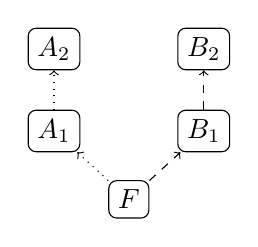
\begin{tikzpicture}[node distance=5mm,
      terminal/.style={rectangle,draw=black,rounded corners=1mm}]
\node (F) [terminal] {$F$};
\node (A1) [terminal,above left=of F] {$A_1$};
\node (A2) [terminal,above=of A1] {$A_2$};
\node (B1) [terminal,above right=of F] {$B_1$};
\node (B2) [terminal,above=of B1] {$B_2$};
\graph {
  (F) ->[dotted] (A1) ->[dotted] (A2);
  (F) ->[dashed] (B1) ->[dashed] (B2);
};
\end{tikzpicture}
\caption{Unslashed Progress Counterexample}\label{fig:unslashed-counterexample}
\end{figure}
The example is shown in Figure~\ref{fig:unslashed-counterexample}.
$F$ is the most recent finalized block, $A_1$ and $B_1$ immediate children of $F$,
and $A_2$ and $B_2$ immediate children (respectively) of $A_1$ and $A_2$.
Half of the validators have voted for the edges $F\!\!\rightarrow\!\! A_1$
and $A_1\!\! \rightarrow\!\! A_2$ (dotted arrows) and the other half of
the validators have voted for $F\!\! \rightarrow\!\! B_1$
and $B_1\!\! \rightarrow\!\! B_2$ (dashed arrows).
It is impossible to make a super-majority link from $F$ to any other block
without some validators being slashed.
A new edge from $F$ to a block one or two levels above $F$ would violate slashing
Condition I, because every validator already has votes with a target at that level.
An edge from $F$ to a block at any higher level would violate Condition II,
with the inner vote being that validator's vote for $A_1\!\! \rightarrow\!\! A_2$
or $B_1\!\! \rightarrow\!\! B_2$.

\section{Instantiating Hypotheses and Parameters}

The definitions and proven properties in the abstract
models of Casper are quite far from those in the Casper paper~\cite{Buterin2017},
partly due to proof engineering concerns described above.
To bring our results closer to the paper, and thus to actual implementations,
we instantiate the key abstractions.
In particular, we assume an arbitrary function which maps validators to their deposits:
\begin{lstlisting}[language=Coq]
Variable deposit : Validator -> nat.
\end{lstlisting}
Using the support for big operators in Mathematical Components~\cite{Bertot2008}, we
then define the total deposits of all validators:
\begin{lstlisting}[language=Coq]
Definition deposits := \sum_(v : Validator) (deposit v).
\end{lstlisting}
We also define a function from a natural number \lstinline{n} to the set of sets of
validators which have total deposit at least \lstinline{n}:
\begin{lstlisting}[language=Coq]
Definition gdset n := [set x in powerset [set: Validator] |
 \sum_(v in x) (deposit v) >= n].
\end{lstlisting}
Writing \lstinline{m %/ d} for the quotient of the Euclidean division of
\lstinline{m} by \lstinline{d}, we define two sets:
\begin{lstlisting}[language=Coq]
Definition deposit_bot := gdset (deposits %/ 3).+1.
Definition deposit_top := gdset ((2 * deposits) %/ 3).+1.
\end{lstlisting}
which allows us to prove:
\begin{lstlisting}[language=Coq]
Lemma deposit_validator_intersection : forall q1 q2,
 q1 \in deposit_top -> q2 \in deposit_top ->
 exists q3, q3 \in deposit_bot /\ q3 \subset q1 /\ q3 \subset q2.
\end{lstlisting}
using the arithmetical lemma
\begin{lstlisting}[language=Coq]
Lemma thirds : forall n, (n %/ 3).+1 + n <= 2 * (2 * n %/ 3).+1.
\end{lstlisting}
This intersection lemma shows that we can instantiate the
abstract \lstinline{quorum_1} and \lstinline{quorum_2}
used in our proofs with specific sets \lstinline{deposit_top}
and \lstinline{deposit_bot}.

\subsection{Block Trees and Transition System}

Working from the other end of the abstraction spectrum, we define
functions and datatypes in Coq resembling those in the beacon chain
implementation~\cite{Beacon}, to be used when defining global system
state and node-local behavior.
In particular, following Toychain, we abstracted a block to a Coq record
type containing, most notably, a hash of the previous block and a collection of attestations
by validators:
\begin{lstlisting}[language=Coq]
Record Attestation := mkAR { distance_src : nat;
 attester : Validator; }.

Record Block := mkB { parent_hash : Hash;
  attestations : seq Attestation;
  distance : nat; }.
\end{lstlisting}
Using notions from the FCSL PCM library~\cite{fcslpcm}, we then define block forests as finite maps
from hashes to blocks:
\begin{lstlisting}[language=Coq]
Definition Blockforest := union_map Hash Block.
\end{lstlisting}
This allows us to instantiate a suitably concrete parent relation over hashes:
\begin{lstlisting}[language=Coq]
Definition hash_parent_bf (bf : Blockforest) : rel Hash :=
[rel x y | (x \in dom bf) && (y \in dom bf) &&
 if find y bf is Some b then parent_hash b == x else false].
\end{lstlisting}
for which we can instantiate the desired hypothesis:
\begin{lstlisting}[language=Coq]
Lemma hash_parent_bf_eq : forall f h1 h2 h3,
 hash_parent_bf f h2 h1 -> hash_parent_bf f h3 h1 -> h2 = h3.
\end{lstlisting}

We can now consider a block forest as a concrete global state, and define
a mapping from from block forests to a \lstinline{vote_msg} function:
\begin{lstlisting}[language=Coq]
Definition vote_msg_bf bf v h distance distance_src : bool :=
 if find h bf is Some b then
  (distance b == distance) &&
  ((mkAR distance_src v) \in attestations b)
 else false.
\end{lstlisting}
The initial state of the system is simply the finite map taking the genesis
block hash to the genesis block:
\begin{lstlisting}[language=Coq]
mkSt (vote_msg_bf (#GenesisBlock \\-> GenesisBlock))
\end{lstlisting}
Finally, we define a transition system that given a block \lstinline{b}, updates
the global state \lstinline{bf} with \lstinline{b}:
\begin{lstlisting}[language=Coq]
mkSt (vote_msg_bf (#b \\-> b \+ bf))
\end{lstlisting}
Accountable safety holds for every state in this transition system, and we
believe it can serve as a specification for the Casper beacon chain
implementation~\cite{Beacon}, and is closer to the level of detail needed
generate a correct-by-construction implementation from the specification.

\subsection{Beacon Node}
The state of the beacon chain~\cite{Beacon} is split into two main parts, an
active state and a crystallized state. The active state is updated every block,
while the crystallized state is only updated corresponding to a cycle length
parameter of the protocol, which is set to 64 slots in the beacon chain
implementation~\cite{Beacon}.

In our Coq formulation, we define the state of a node in the beacon chain as a
record containing the blockforest and this beacon chain state.
It also includes other parameters of the system, such as the cycle length
mentioned above.
\begin{lstlisting}[language=Coq]
Record State {Hash : ordType} :=
  Node {
    id : NodeId;
    peers : peers_t;
    blocks : Blockforest;
    cstate : @CrystallizedState Hash;
    astate : @ActiveState Hash;
    (* set to 1024 shards, see beacon chain implementation *)
    shardCount : nat;
    (* set to 64 slots, see beacon chain implementation *)
    cycleLength : nat;
  }.
\end{lstlisting}
When a block arrives on a node, the crystallized and active states are updated
via the state transition function specified in~\cite{Beacon}. The update of the
crystallized state is where most of the Casper functionality occurs. Should the
slot number of the block be at least 64 past the last recalculation slot, the
crystallized state is updated by applying the rewards and penalties for the
validators, as well as managing the justification and finalization of blocks.
For example, the Coq code for the state update has functions such as
\lstinline{applyRewardsAndPenalties} below, which calculates and updates the
balances for all active validators given the current state and block.

\begin{lstlisting}[language=Coq]
Definition applyRewardsAndPenalties
           (crystallizedState :
              @CrystallizedState [ordType of Hash])
           (activeState : @ActiveState [ordType of Hash])
           (blk : block)
           (cycleLength : nat) :=
  (* ... omitted ... *)
\end{lstlisting}
In addition to updating the crystallized and active states, the arrived block is
also appended to the block forest, and the new state is returned, along with a
message from the node that received the block to all of its peers.

\begin{lstlisting}[language=Coq]
Definition procInt (st : @State [ordType of Hash])
           (tr : InternalTransition) (ts : Timestamp) :=
 let: Node n prs bf cst ast cl := st in
 match tr with
 | BlockT b =>
   let: parentBlock := get_block bf (parent_hash b) in
   let: (crystallizedState, activeState) :=
      computeStateTransition cst ast parentBlock b cl in
   let: newBf := bfExtend bf b in
   pair (Node n prs newBf crystallizedState activeState cl)
        (emitBroadcast n prs (BlockMsg b))
 end.
\end{lstlisting}
These definitions tighten the correspondence between our Coq code and the Beacon
chain implementation in~\cite{Beacon}. Along with our abstract safety and
liveness proofs, these definitions will allow us to perform verification at this
low level, providing as much assurance as possible for the correctness of the
Casper protocol.

\section{Conclusion}
\label{sec:conclusion}

%Ongoing refinements include aligning the Toychain concept of a fork,
%which is in terms of block sequence prefixing, with the more abstract Casper
%notion of a fork in terms of finalized blocks over the closure of the parent
%hash relation.

We presented a formalization of Casper in Coq, and proofs of accountable safety
and plausible liveness.
These proofs clarified the assumptions needed for the properties stated in
the Casper paper~\cite{Buterin2017}, especially what assumptions on
validator behavior are needed for plausible liveness.
Our formalization work paves the way for transferring accountable safety and
plausible liveness from Hirai's abstract models to hold for steps over the
Toychain global state according to a step relation and node state definition
matching those in the Ethereum reference beacon chain node
implementation~\cite{Beacon}.

%Ultimately, we aim to transfer accountable safety and plausible liveness from
%Hirai's abstract models to hold for steps over the Toychain global state according to a step
%relation and node state definition matching those in the Ethereum reference beacon
%chain node implementation~\cite{Beacon}.
%
%That is, we will express and prove both properties
%along the lines of the \emph{clique consensus} property in Toychain~\cite{Pirlea2018}, i.e., similarly to
%\begin{lstlisting}[language=Coq]
%Theorem accountable_safety_inv : forall (w w' : World),
% accountable_safety w -> step w w' -> accountable_safety w'.
%\end{lstlisting}
%We then plan to use the step relation as a basis for a verified
%node implementation. We also want to capture \emph{sharded} systems,
%which consist of many separate blockchains for reasons of scalability~\cite{sharding}, and to keep up with the Casper protocol design, which is a moving target.

%\begin{lstlisting}[language=Coq]
%Theorem plausible_liveness : forall (w w' : World),
% accountable_safety w -> exists w', step w w' /\ new_justified w w'.
%\end{lstlisting}

%Our goal is to have our Coq implementation correspond as closely as
%possible with the implementation in~\cite{Beacon}. This gives us the greatest
%assurance that our proven properties hold in the most up-to-date Casper version.

%\begin{lstlisting}[language=Coq]
%Definition fork (bc1 bc2 : seq T) :=
% ~ (is_prefix bc1 bc2 \/ is_prefix bc2 bc1).
%\end{lstlisting}

%\section{Discussion}

%% Acknowledgments
%\begin{acks}                            %% acks environment is optional
%                                        %% contents suppressed with 'anonymous'
%  %% Commands \grantsponsor{<sponsorID>}{<name>}{<url>} and
%  %% \grantnum[<url>]{<sponsorID>}{<number>} should be used to
%  %% acknowledge financial support and will be used by metadata
%  %% extraction tools.
%  This material is based upon work supported by the
%  \grantsponsor{GS100000001}{National Science
%    Foundation}{http://dx.doi.org/10.13039/100000001} under Grant
%  No.~\grantnum{GS100000001}{nnnnnnn} and Grant
%  No.~\grantnum{GS100000001}{mmmmmmm}.  Any opinions, findings, and
%  conclusions or recommendations expressed in this material are those
%  of the author and do not necessarily reflect the views of the
%  National Science Foundation.
%\end{acks}


%% Bibliography
\bibliography{bib}


%% Appendix
%\appendix
%\section{Appendix}
%
%Text of appendix \ldots

\end{document}
